%%%%%%%%% begin snippet
%% You need to add the package "tabularx".
%% Place the snippet right after \begin{document}

% need tabularx
\documentclass{article}
\usepackage{tabularx}
\usepackage{graphicx}
\usepackage{pdfpages}
\usepackage{listings}
\usepackage{subcaption}
\usepackage{verbatim}

\begin{document}
    \begin{titlepage}
           \begin{center}
                 \begin{huge}
                       %% Update assignment number here
                       \textbf{Assignment 2}
                 \end{huge}
           \end{center}

           \begin{center}
                 \begin{large}
                       Machine Learning 1, SS23
                 \end{large}
           \end{center}

           \begin{center}
                \begin{tabularx}{\textwidth}{|>{\hsize=.33\hsize}X|>{\hsize=.33\hsize}X|>{\hsize=.33\hsize}X|}

                       \hline
                       \multicolumn{3}{|c|}{\textbf{Team Members}} \\
                       \hline
                       Last name & First name & Matriculation Number \\
                       \hline
                       Grassl & Ifeoma & 12011965 \\
                       \hline
                       Royer & Christoph & 12004184 \\
                       \hline

                \end{tabularx}
           \end{center}

    \end{titlepage}

    \section{Neural Networks}
    \subsection{PCA and Classification}
    \subsubsection{PCA for dimensionality reduction}
    \textit{For implementation see } \texttt{nn\_classification.py}.

    We used $320$ components, which gave a ratio of $95.05\%$ explained variance.

    \subsubsection{Varying the number of hidden neurons}
    \textit{For implementation see } \texttt{nn\_classification.py}.

    \textbf{Output of the program:}
    \begin{lstlisting}
Number of hidden neurons: 2
Train accuracy: 0.5913. Test accuracy: 0.4262
Loss: 1.0635
Number of hidden neurons: 10
Train accuracy: 0.9982. Test accuracy: 0.7215
Loss: 0.0156
Number of hidden neurons: 100
Train accuracy: 1.0000. Test accuracy: 0.7724
Loss: 0.0054
Number of hidden neurons: 200
Train accuracy: 1.0000. Test accuracy: 0.7918
Loss: 0.0044
    \end{lstlisting}

    Underfitting is generally easy to spot, as it manifests in poor performance both on training and on test data.
    This is often the case if the model does not have enough capacity (ie. not enough complexity); in this case, the loss converges on a bad value.
    The model cannot improve past a (relatively bad) optimum.

    Overfitting takes place when a powerful model is trained on too little data.
    In this case, the model learns the training data -- including its inaccuracies -- too well.
    The side effect of this is that the model fails to predict test data accurately because of an overfixation on the particularities of the training dataset.

    We could not detect overfitting in this example.
    Thus we chose the model with $200$ hidden neurons, as it had the best test accuracy.

    \subsubsection{Preventing overfitting}
    Our preliminary guess was that model \textbf{c} -- with \textit{alpha} = $0.1$ and \textit{early\_stopping} = True -- would work best.
    The reasoning was that multiple prevention mechanisms would be best at catchinng overfitting.

    It turns out that model \textbf{a} -- with only \textit{alpha} = $0.1$ -- worked best.

    \pagebreak
    We can see the test output here -- note that Variation 0 (model \textbf{a}) improved on the test accuracy from the previous task:

    \begin{lstlisting}
Number of hidden neurons: 200
Variation 0:
Train accuracy: 1.0000. Test accuracy: 0.8378
Loss: 0.0678
Variation 1:
Train accuracy: 0.9770. Test accuracy: 0.7700
Loss: 0.0541
Variation 2:
Train accuracy: 0.9709. Test accuracy: 0.7772
Loss: 0.1722
    \end{lstlisting}

    \subsubsection{Variability of the performance}
    \textit{For implementation see } \texttt{nn\_classification.py}.

    We chose model \textbf{a}, as it showed the best output.
    Note that this is a form of overfitting, as we are choosing hyperparameters based on their performance on the test set,
    but the assignment requires this.

    The implementation outputs the following:
    \begin{lstlisting}
Seed: 12011965
Train accuracy: 1.0000. Test accuracy: 0.8354
Loss: 0.0668
Seed: 12004184
Train accuracy: 1.0000. Test accuracy: 0.8475
Loss: 0.0656
Seed: 1234
Train accuracy: 1.0000. Test accuracy: 0.8402
Loss: 0.0672
Seed: 7
Train accuracy: 1.0000. Test accuracy: 0.8402
Loss: 0.0673
Seed: 4321
Train accuracy: 1.0000. Test accuracy: 0.8329
Loss: 0.0671
Train accuracy overall:
On the train set: 1.0000 +/- 0.0000 [1.0000:1.0000]
On the test set: 0.8392 +/- 0.0050 [0.8329:0.8475]
    \end{lstlisting}

    Changing the seed changes the pseudo-random initial state of the MLP.
    This should not change the optimal solution,
    but a fortunate choice of the initial state may drastically reduce the number of iterations needed for convergence.

    \subsubsection{Loss curve}
    We chose seed $12004184$, as it showed the best performance in the previous test.
    Note that this is again a form of overfitting, but the assignment requires this.

    
\includegraphics[width=\textwidth]{code/plots/losscurve}

    \pagebreak
    \subsubsection{Prediction on the test set}
    The following is the output of the trained model's prediction and the confustion matrix on the test set:

    \begin{lstlisting}
Predicting on the test set
        precision recall    f1-score    support

0       0.77      0.85      0.81        40
1       0.83      0.91      0.87        44
2       0.85      0.73      0.79        48
3       0.79      0.79      0.79        39
4       0.82      0.89      0.86        37
5       0.80      0.84      0.82        43
6       0.79      0.68      0.73        44
7       0.94      0.86      0.90        37
8       0.71      0.80      0.75        30
9       0.98      0.96      0.97        51

accuracy                           0.83       413
macro avg       0.83      0.83      0.83       413
weighted avg       0.84      0.83      0.83       413

[[34  0  0  0  2  2  1  0  0  1]
 [ 1 40  0  1  0  0  2  0  0  0]
 [ 0  2 35  3  1  3  0  0  4  0]
 [ 1  0  0 31  1  0  2  0  4  0]
 [ 0  1  0  0 33  1  1  0  1  0]
 [ 1  2  1  0  1 36  2  0  0  0]
 [ 4  2  2  3  0  3 30  0  0  0]
 [ 3  0  1  0  0  0  0 32  1  0]
 [ 0  0  2  1  2  0  0  1 24  0]
 [ 0  1  0  0  0  0  0  1  0 49]]

    \end{lstlisting}
    \textit{Recall} measures the ratio of true positive classifications in relation to the amount of samples that were available for given class.
    It thus measures how many samples were missed to be recognised as members of the class.
    We can easily recalculate this for class $i$ with $\frac{tp_i}{support_i}$, with $tp_i$ being the $i$th diagonal entry in the confusion matrix (= true positive classification).

    The class with the lowest recall is thus the one where its instances are most often recognised as members of a different class.
    In our example, this was the digit 6; images representing a 6 were most often classified as other digits compared to all the other digits.
    We were able to conclude that because the recall for class 6 was the lowest with $0.68$.


    \subsection{Model selection using GridSearch}
    \subsubsection{Parameter space}

    \textit{For implementation see } \texttt{nn\_classification.py}.

    The parameter space spans the cross product of all the options, thus there are
    $4 * 2 * 2 * 2 = 32$ possible architectures.

    \subsubsection{Implementation}

    \textit{For implementation see } \texttt{nn\_classification.py}.

    \subsubsection{Best parameter set}

    \textit{For implementation see } \texttt{nn\_classification.py}.

    The \textit{GridSearchCV} comes to the following best solution:

    \begin{lstlisting}
Best score: 0.8477
Best parameters: {'activation': 'relu', 'alpha': 1.0, 'hidden_layer_sizes': (100,), 'solver': 'lbfgs'}
    \end{lstlisting}

    \subsubsection{Best test score}

    \textit{For implementation see } \texttt{nn\_classification.py}.

    The best estimator of the grid search has the following score on the test set:
    \begin{lstlisting}
Score of best estimator on test set: 0.8716
    \end{lstlisting}

    \subsubsection{Hyperparameters vs. model parameters}
    What makes hyperparameters special is that they inform they affect the model in such a way that they cannot be changed during training.
    This could be because it changes the available set of model parameters (eg. different sizes of hidden layers),
    or because it changes the interpretation of the model parameters (eg. different activation functions).
    In contrast to parameters of neural networks (eg. perceptron weights and intercepts),
    hyperparameters (such as activation function, solver) are often categorical and thus could be used for gradient descent at all.

    \pagebreak
    
    \section{Regression with Neural Networks}
    \subsection{Implement the function $calculate\_mse$}

    This function is used to compute the mean squared error between the target values and the corresponding predicted values obtained from a model. The MSE is a commonly used metric to evaluate the performance of regression models.
    Code:
    \begin{lstlisting}
    def calculate_mse(targets, predictions):
        """
        :param targets:
        :param predictions: Predictions obtained by using the model
        :return:
        """
        mse = mean_squared_error(targets, predictions)
    return mse
    \end{lstlisting}
    \subsection{Train the network to solve the task: Using $GridSearchCV$ to find a good model}
    We chose a similar dictionary as in task 1:
    \begin{lstlisting}
    parameters = {
        "alpha": [0.0, 0.1, 1.0],
        "solver": ["lbfgs", "adam"],
        "activation": ["logistic", "relu"],
        'early_stopping': [True, False],
        "hidden_layer_sizes": [(100, ), (200, ), (300, ), (400, )]
    }
    \end{lstlisting}
    It tests 3 different alpha values, i.e. regularization strengths, two different solvers/ optimizers, two activations, combinations with early stopping being enabled and not enabled, and it tests four different hidden layer sizes. Which means the grid\_search will test out 3*2*2*2*4=96 different architectures.\\
    The best model ended up having the following parameters:
    \begin{lstlisting}
        Best parameters: {'activation': 'relu', 'alpha': 0.1, 'early_stopping': True, 'hidden_layer_sizes': (400,), 'solver': 'lbfgs'}
    \end{lstlisting}
    \subsection{Report the train and test loss}
    We are using the $calculate\_mse$ function from above to calculate the mean squared error loss. Result:
    \begin{lstlisting}
        Train MSE: 0.0008. Test MSE: 0.0009
    \end{lstlisting}

    \pagebreak

    \section{Bonus: Implementation of a Perceptron}
    \subsection{ Plots of the decision boundaries learned for the two datasets, two implementations, and different values of learning rates and number of iterations}
    \subsubsection{Linearly separable dataset, $learning\_rate=0.1$, $iterations=5$}
    
    \begin{figure}[ht]
        \centering
        \begin{subfigure}{0.4\textwidth}
            \centering
            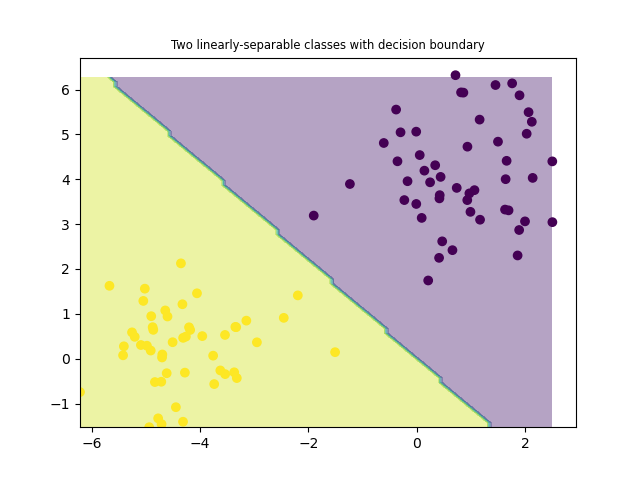
\includegraphics[width=\linewidth]{code/plots/our_perceptron_LR0.1_ITER5_dataset_loaddata}
            \caption{Our Perceptron}
            \label{fig:image1}
        \end{subfigure}
        \hspace{2cm} % Adjust the horizontal spacing between the subfigures
        \begin{subfigure}{0.4\textwidth}
            \centering
            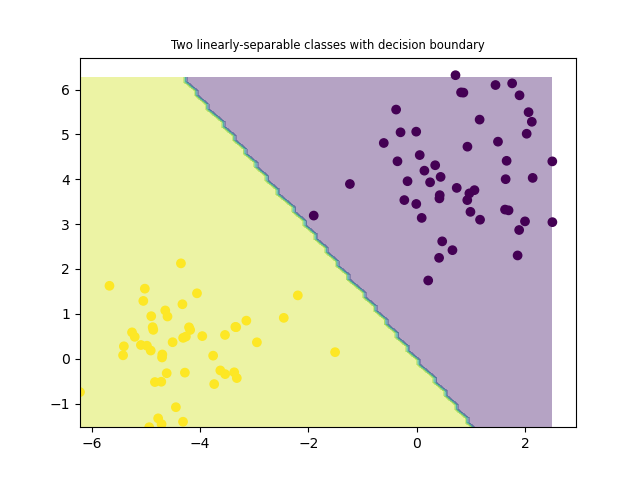
\includegraphics[width=\linewidth]{code/plots/SKperceptron_LR0.1_ITER5_dataset_loaddata}
            \caption{SKperceptron}
            \label{fig:image2}
        \end{subfigure}
        \label{fig:overall}
    \end{figure}

    \begin{verbatim}    
        Our perceptron:                       Sklearn perceptron:
        Training MSE: 0.0                     Training MSE: 0.0
        Testing MSE:  0.0                     Testing MSE: 0.0
        train error: 0.0                      train error: 0.0
        test error: 0.0                       test error: 0.0
    \end{verbatim}

    \subsubsection{Linearly separable dataset, $learning\_rate=0.001$, $iterations=1$}

    \begin{figure}[ht]
        \centering
        \begin{subfigure}{0.4\textwidth}
            \centering
            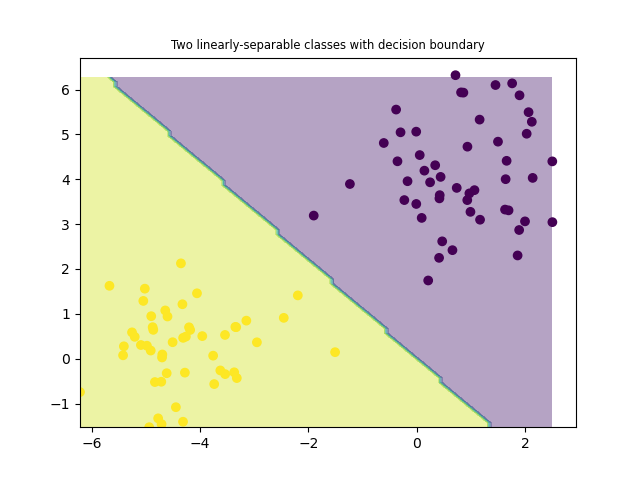
\includegraphics[width=\linewidth]{code/plots/our_perceptron_LR0.001_ITER1_dataset_loaddata}
            \caption{Our Perceptron}
            \label{fig:image1}
        \end{subfigure}
        \hspace{2cm} % Adjust the horizontal spacing between the subfigures
        \begin{subfigure}{0.4\textwidth}
            \centering
            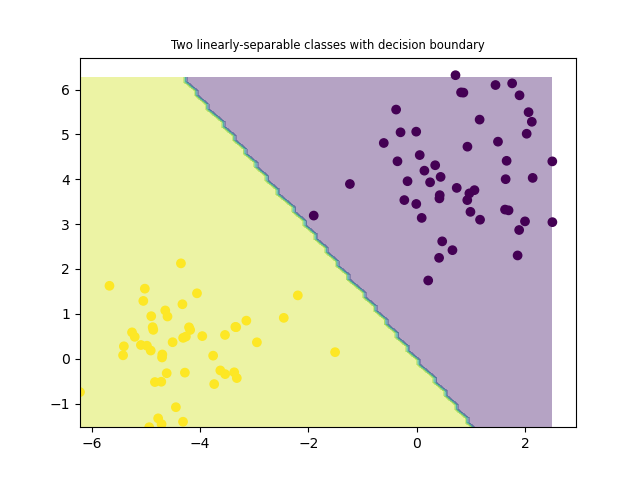
\includegraphics[width=\linewidth]{code/plots/SKperceptron_LR0.001_ITER1_dataset_loaddata}
            \caption{SKperceptron}
            \label{fig:image2}
        \end{subfigure}
        \label{fig:overall}
    \end{figure}

    \begin{verbatim}    
        Our perceptron:                       Sklearn perceptron:
        Training MSE: 0.0                     Training MSE: 0.0
        Testing MSE:  0.0                     Testing MSE: 0.0
        train error: 0.0                      train error: 0.0
        test error: 0.0                       test error: 0.0
    \end{verbatim}

    \subsubsection{Non linearly separable dataset, $learning\_rate=0.001$, $iterations=1$}

    \begin{figure}[ht]
        \centering
        \begin{subfigure}{0.4\textwidth}
            \centering
            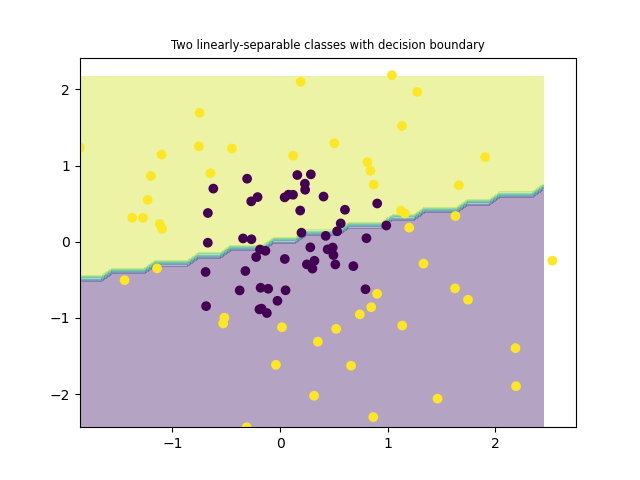
\includegraphics[width=\linewidth]{code/plots/our_perceptron_LR0.001_ITER1_dataset_load_non_linearly_separable_data}
            \caption{Our Perceptron}
            \label{fig:image1}
        \end{subfigure}
        \hspace{2cm} % Adjust the horizontal spacing between the subfigures
        \begin{subfigure}{0.4\textwidth}
            \centering
            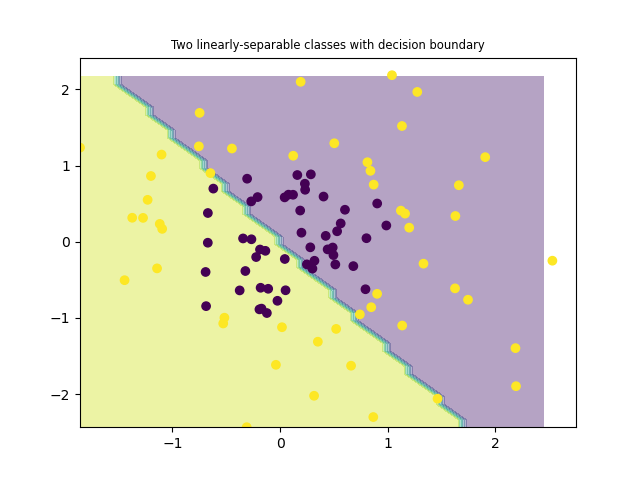
\includegraphics[width=\linewidth]{code/plots/SKperceptron_LR0.001_ITER1_dataset_load_non_linearly_separable_data}
            \caption{SKperceptron}
            \label{fig:image2}
        \end{subfigure}
        \label{fig:overall}
    \end{figure}

    \begin{verbatim}    
        Our perceptron:                        Sklearn perceptron:
        Training MSE: 0.475                    Training MSE: 0.45
        Testing MSE:  0.47                     Testing MSE: 0.5
        train error: 0.475                     train error: 0.45
        test error: 0.47                       test error: 0.5
    \end{verbatim}

    \subsubsection{Non linearly separable dataset, $learning\_rate=0.1$, $iterations=5$}

    \begin{figure}[ht]
        \centering
        \begin{subfigure}{0.4\textwidth}
            \centering
            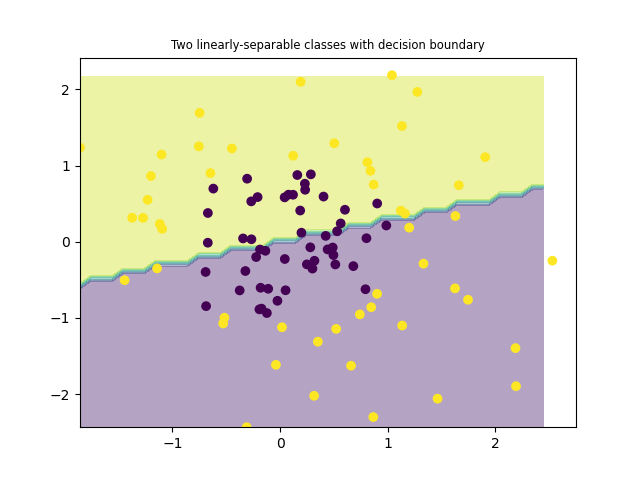
\includegraphics[width=\linewidth]{code/plots/our_perceptron_LR0.1_ITER5_dataset_load_non_linearly_separable_data}
            \caption{Our Perceptron}
            \label{fig:image1}
        \end{subfigure}
        \hspace{2cm} % Adjust the horizontal spacing between the subfigures
        \begin{subfigure}{0.4\textwidth}
            \centering
            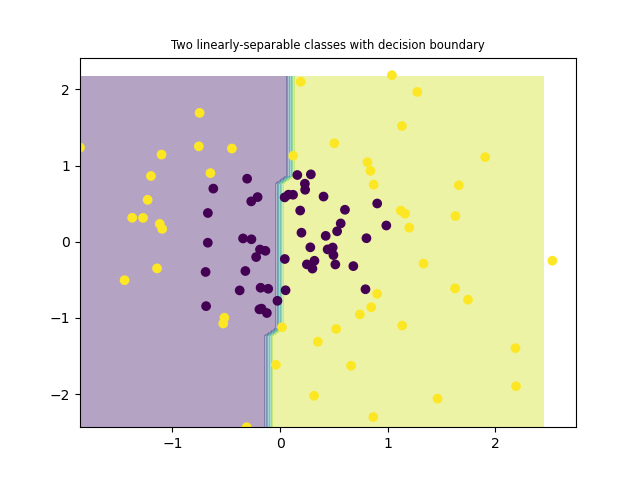
\includegraphics[width=\linewidth]{code/plots/SKperceptron_LR0.1_ITER5_dataset_load_non_linearly_separable_data}
            \caption{SKperceptron}
            \label{fig:image2}
        \end{subfigure}
        \label{fig:overall}
    \end{figure}

    \begin{verbatim}    
        Our perceptron:                        Sklearn perceptron:
        Training MSE: 0.4625                    Training MSE: 0.475
        Testing MSE:  0.45                     Testing MSE: 0.5
        train error: 0.4625                     train error: 0.475
        test error: 0.45                       test error: 0.5
    \end{verbatim}

    \subsubsection{Non linearly separable dataset, $learning\_rate=0.0001$, $iterations=10000$}

    \begin{figure}[ht]
        \centering
        \begin{subfigure}{0.4\textwidth}
            \centering
            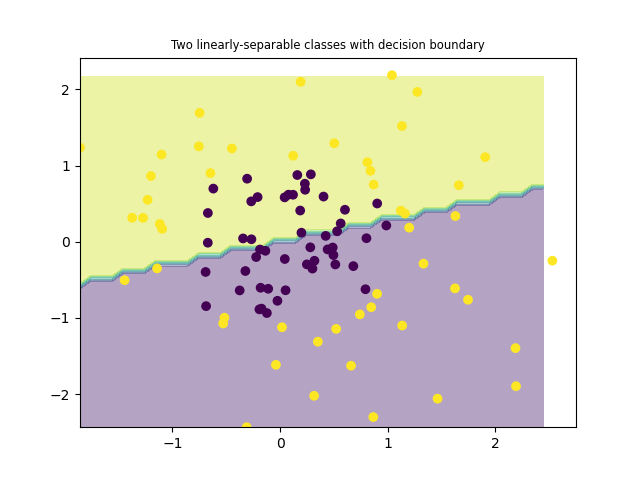
\includegraphics[width=\linewidth]{code/plots/our_perceptron_LR0.0001_ITER10000_dataset_load_non_linearly_separable_data.png}
            \caption{Our Perceptron}
            \label{fig:image1}
        \end{subfigure}
        \hspace{2cm} % Adjust the horizontal spacing between the subfigures
        \begin{subfigure}{0.4\textwidth}
            \centering
            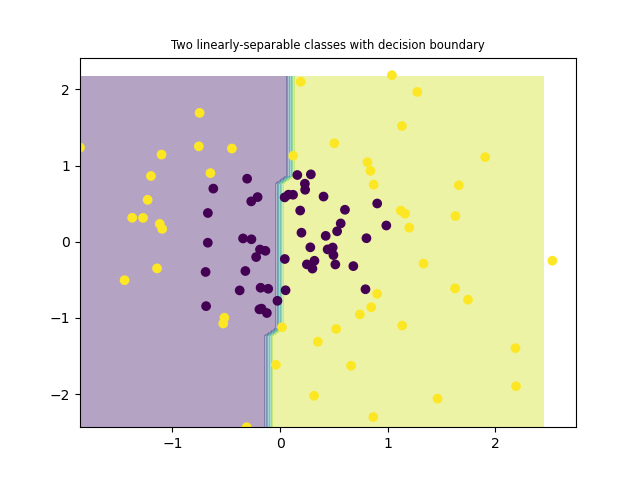
\includegraphics[width=\linewidth]{code/plots/SKperceptron_LR0.0001_ITER10000_dataset_load_non_linearly_separable_data.png}
            \caption{SKperceptron}
            \label{fig:image2}
        \end{subfigure}
        \label{fig:overall}
    \end{figure}

    \begin{verbatim}    
        Our perceptron:                        Sklearn perceptron:
        Training MSE: 0.4625                    Training MSE: 0.475
        Testing MSE:  0.45                     Testing MSE: 0.45
        train error: 0.4625                     train error: 0.475
        test error: 0.45                       test error: 0.45
    \end{verbatim}

    \subsection{How do the results of sklearn implementation of Perceptron differ from your implementation?}

    The results for the linearly separable dataset do not differ. For the Non linearly separable dataset it's clear to see that the decision boundary changes a lot more than with our implementation, although the results for the mean squared error losses and the classification errors are very similar.

    \subsection{How many training iterations does it take for the perceptron to learn to classify all training samples perfectly?}

    For the linearly separable dataset it takes our perceptron two full iterations to classify all training samples perfectly (for the values of learning\_rate that we tested). However, even only one iteration also leads to a 0.0 training and testing MSE as well as a 0.0 train and test error (with about two samples being incorrectly classified)\\
    For the non linearly separable dataset it didn't matter how high we made the learning rate, there always ended up being 30 or so samples that were incorrectly classified.

    \subsection{What is the misclassification rate (the percentage of incorrectly classified examples) for both datasets?}

    I have added the misclassification rate in subsection 3.1 (test error and train error)
    For the linearly separable dataset it is 0.0 while for the non linearly separable dataset it is between 0.45 and 0.47 for the test error.

    \subsection{How would you learn a non-linear decision boundary using a single perceptron? (Hint: recall what we had for linear regression.)}

    To learn non-linear decision boundaries, you would typically need a multi-layer perceptron. The additional hidden layers in an MLP allow for the extraction of non-linear features from the input data, enabling the network to learn and represent more complex decision boundaries. The key is to transform the input features into a higher-dimensional space where a linear decision boundary can be established (feature engineering).
    You can creating new features or modifying existing features to improve the performance and effectiveness of a machine learning model.


\end{document}

%%%%%%%%% end snippet
